% !TeX encoding = UTF-8
%



\newpage



\phantomsection
\label{Abschnitt:Tests:Protokoll:Extrem}



\subsection*{Extremtests}


Zunächst haben wir eine Hilfsklasse für einfaches Benchmarking geschrieben. Diese misst die Ausführungszeit für eine C\#-Methode. Dies findet mit einer bestimmten Anzahl an Wiederholungen statt, die als Eingabe festgelegt werden kann. Dieser Ansatz liefert jedoch nur begrenzt Aussagen über die Performance, da hier die Grafischen Ausgaben nicht mit berücksichtigt werden. Aus diesem Grund haben wir ein etwas ausgefeilteres Programm geschrieben, wo auch die grafischen Ausgaben berücksichtigt werden. Dabei verwenden wir ein weiteres Werkzeug: MonoDevelop, da der Test lediglich für Mono geschrieben wurde.\\~\\


\phantomsection
\label{Abschnitt:Tests:Protokoll:Extrem:Knoten_Erzeugen}

\begin{description}

	\item[ET\_1] \textit{Erzeugen großer Knoten}\hfill\\
	
\end{description}


\begin{figure}[ht]

	\centering
	\label{Anhang:Medien:Travelmate}
	
	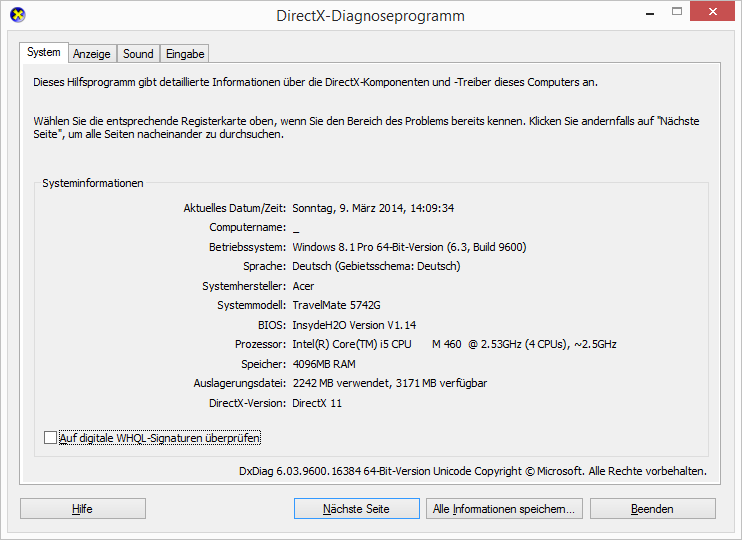
\includegraphics[width=0.9\textwidth]{\Media/Travelmate.png}
	
	\caption{Systemeigenschaften.}

\end{figure}

~\\

Unsere Benchmark-Klasse ohne Grafik-Ausgabe liefert beim Erzeugen quadratischer Knoten unterschiedlicher Größen:\\~\\

\noindent
min: Kürzeste Zeit, max: Längste Zeit, avg: Mittlere zeit, out: Erster Ausreißer/Caching.\\


\noindent
Knoten-Erzeugen: Knoten mit 100 Kanten, 100 WH:\\
max = 600210 NS >= 0 MS >= 0 S\\
min = 57915 NS >= 0 MS >= 0 S\\
avg = 78165 NS >= 0 MS >= 0 S\\
out = 50158035 NS >= 50 MS >= 0 S\\
~\\
Knoten-Erzeugen: Knoten mit 1000 Kanten, 1000 WH:\\
max = 2246940 NS >= 2 MS >= 0 S\\
min = 532575 NS >= 0 MS >= 0 S\\
avg = 607905 NS >= 0 MS >= 0 S\\
out = 56641680 NS >= 56 MS >= 0 S\\
~\\
Knoten-Erzeugen: Knoten mit 10000 Kanten, 10000 WH:\\
max = 19330650 NS >= 19 MS >= 0 S\\
min = 5473980 NS >= 5 MS >= 0 S\\
avg = 7617240 NS >= 7 MS >= 0 S\\
out = 54172395 NS >= 54 MS >= 0 S\\
~\\~\\

\noindent
Knoten-Laden: Knoten mit 100 Kanten, 100 WH:\\
max = 1639440 NS >= 1 MS >= 0 S\\
min = 666630 NS >= 0 MS >= 0 S\\
avg = 913275 NS >= 0 MS >= 0 S\\
out = 62651880 NS >= 62 MS >= 0 S\\
~\\
Knoten-Laden: Knoten mit 1000 Kanten, 100 WH:\\
max = 7217100 NS >= 7 MS >= 0 S\\
min = 4754295 NS >= 4 MS >= 0 S\\
avg = 5197365 NS >= 5 MS >= 0 S\\
out = 80073360 NS >= 80 MS >= 0 S\\
~\\
Knoten-Laden: Knoten mit 10000 Kanten, 100 WH:\\
max = 93382065 NS >= 93 MS >= 0 S\\
min = 64106235 NS >= 64 MS >= 0 S\\
avg = 69729660 NS >= 69 MS >= 0 S\\
out = 148111740 NS >= 148 MS >= 0 S\\
~\\

\noindent
Unter Berücksichtigung der grafischen Ausgabe dauerte das  Erzeugen von Knoten mit ...\\

\noindent
... 500 Kanten: Zwischen 15 und 19 MS.\\
... 1000 Kanten: Zwischen 27 und 32 MS.\\
... 5000 Kanten: Zwischen  und  MS.\\
... 10000 Kanten: $\infty$ MS.


